\documentclass{lehramt-informatik-minimal}
\InformatikPakete{er,syntax}
\begin{document}

\section{Zirkus}

\begin{quellen}
\item \cite[Seite 1-2, Aufgabe 1: ER-Diagramm Einstieg]{db:pu:1}
\item \cite[Seite 11, Thema Nr. 2, Aufgabe 2: Relationales Modell]{examen:66116:2018:03}
\item \cite[Seite 6, Aufgabe 2, I. Das Entity-Relationship Modell]{examen:66114:2008:03}
\end{quellen}

Das Fremdenverkehrsamt will sich einen besseren Überblick über Zirkusse
verschaffen. In einer Datenbank sollen dazu die Zirkusse, die
angebotenen Vorstellungen, die einzelnen Darbietungen in einer
Vorstellung sowie die zugehörigen Dompteure und Tiere verwaltet werden.

Ein Zirkus wird durch seinen Namen gekennzeichnet und hat einen
Besitzer. Vorstellungen haben eine \texttt{VorstellungsID} und ein
Datum. Darbietungen haben neben der eindeutigen \texttt{ProgrammNr} eine
Uhrzeit. Ein Dompteur hat eine eindeutige \texttt{AngestelltenNr} sowie
einen Künstlernamen. Tiere sind eindeutig durch eine TierNr bestimmt und
haben außerdem eine Bezeichnung der Tierart.

Ein Zirkus bietet Vorstellungen an und stellt Dompteure an. Eine
Darbietung findet in einer Vorstellung statt. Des weiteren trainiert ein
Dompteur Tiere. In einer Darbietung tritt ein Dompteur mit Tieren auf.

\begin{enumerate}
\item 1.1

\begin{enumerate}

%%
% (a)
%%

\item Listen Sie die Entity-Typen und die zugehörigen Attribute auf.

\begin{minted}{md}
* Zirkusse (Zirkus-Nummer, Namen)
  * Besitzer
  * Namen

* Vorstellungen (VorstellungsID)
  * VorstellungsID
  * Datum

* Darbietungen (ProgrammNr)
  * ProgrammNr
  * Datum

* Dompteuere (AngestelltenNr)
  * AngestelltenNr
  * Künstlernamen

* Tiere (TierNr)
  * TierNr
  * Tierart
\end{minted}

%%
%(b)
%%

\item Bestimmen Sie zu jedem Entity-Typen einen Schlüssel.
Fügen Sie, wenn nötig einen künstlichen Schlüssel hinzu.

\begin{minted}{md}
Zirkus (ZID, Besitzer, Name)
Vorstellung (VorstellungsID, Datum, ZID[Zirkus])
Darbietung (ProgrammNr, VorstellungsID[Vorstellung], Uhrzeit)
Dompteur (AngestelltenNr, Kuenstlername, ZID[Zirkus])
Tier (TierNr, Tierart)

trainiert (AngestelltenNr[Dompteur], TierNr[Tier])
trittAuf (AngestelltenNr[Dompteur], TierNr[Tier], ProgrammNr[Darbietung], VorstellungsID[Vorstellung])
\end{minted}

%%
% (c)
%%

\item Erstellen Sie das ER-Diagramm!

Vorstellungen werden von genau einem Zirkus angeboten. Ein Zirkus bietet
mehrere Vorstellungen an und stellt mehrere Dompteure an. Ein Dompteur
ist genau bei einem Zirkus angestellt. Eine Darbietung findet in einer
bestimmten Vorstellung statt. Des weiteren trainiert ein Dompteur
mehrere Tiere, ein Tier kann allerdings auch von mehreren Dompteuren
trainiert werden. In einer Darbietung tritt genau ein Dompteur mit
mindestens einem Tier auf.
\end{enumerate}

\item 1.2 Ergänzen Sie die Funktionalitäten im ER-Diagramm.

Vorstellungen werden von genau einem Zirkus angeboten. Ein Zirkus bietet
mehrere Vorstellungen an und stellt mehrere Dompteure an. Ein Dompteur
ist genau bei einem Zirkus angestellt. Eine Darbietung findet in einer
bestimmten Vorstellung statt. Des weiteren trainiert ein Dompteur
mehrere Tiere, ein Tier kann allerdings auch von mehreren Dompteuren
trainiert werden. In einer Darbietung tritt genau ein Dompteur mit
mindestens einem Tieren auf.

\item 1.3

\begin{enumerate}

%%
% (a)
%%

\item Was bedeutet „mehrere“?

%%
% (b)
%%

\item Ergänzen Sie die Kardinalitäten in min-max Notation im
ER-Diagramm.

\end{enumerate}

\end{enumerate}

%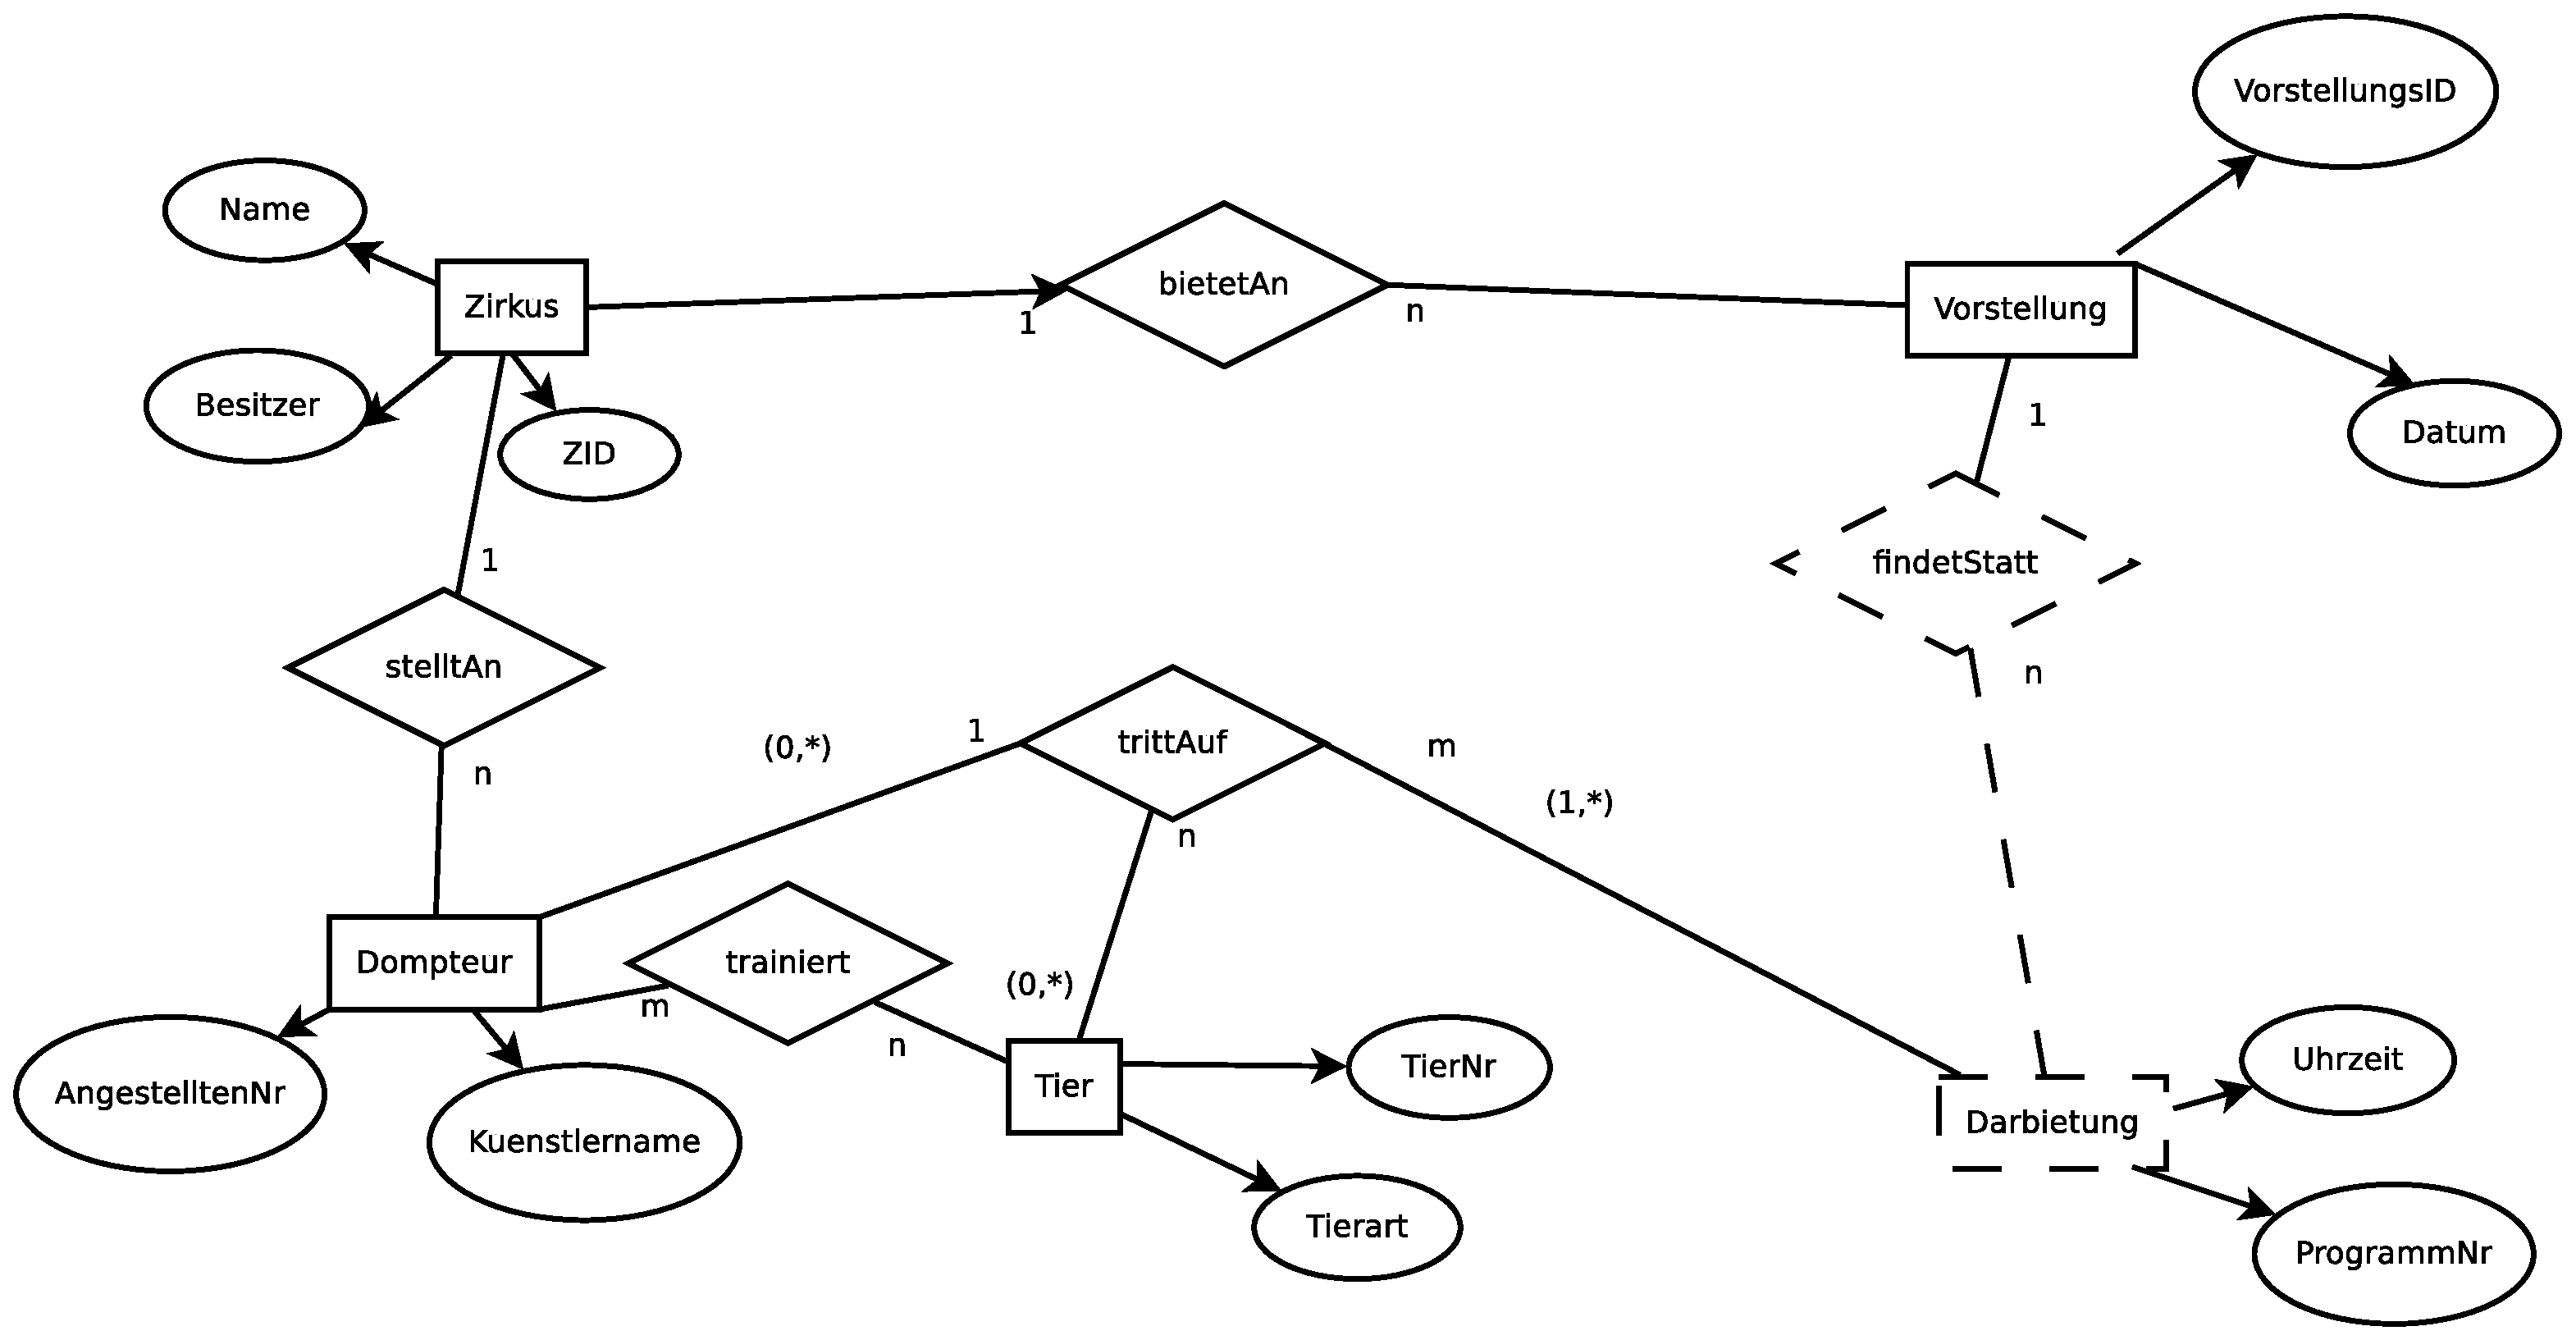
\includegraphics[width=\linewidth]{Zirkus.eps}
\end{document}
